\subsection{Comparison to chemiluminescence measurement}
\label{sec:cld}

After having assured the functionality of our converter in the lab
setting, we wanted to use it in ambient air. There we had to struggle
with additional challenges. First and foremost the concept our setup
allows us only to measure \ch{NO2} or \ch{NO_x} directly, but not
\ch{NO}. Only in our very special \ch{NO2} free setting, could we
determine the Nitrogen Monoxide concentration directly. In this more
general setting we chose the strategy of measuring \ch{NO2} and
\ch{NO_x} alternatingly, i.\,e.\ we measured a \ch{NO2} spectrum, then
added Ozone to the sample air, waited for \SI{30}{\second} to make
sure the cavity was purged, took a \ch{NO_x} spectrum, switched of the
Ozone stream and purged again for \SI{30}{\second}. In the evaluation
step we then interpolated the \ch{NO2} concentrations and subtract
them from the \ch{NO_x} concentration. 

This procedure drastically reduces the time resolution and leads to
ohter complications. Depending on the location the \ch{NO_x}
concentration and composition can fluctuate strongly during
\SI{30}{\second}. This contests the validity of our algorithm and
indeed repeatedly lead to `negative' \ch{NO} concentrations. One
loophole is to increase the averaging time further and only compare
\SI{30}{\minute} averages of \ch{NO_x} and \ch{NO2}. Depending on the
circumstances this can be acceptable for stationary measurements, however


\subsubsection{Setup}
\label{sec:cld-setup}

\subsubsection{Results}
\label{sec:cld-results}

\begin{figure}[htbp]
  \centering
  %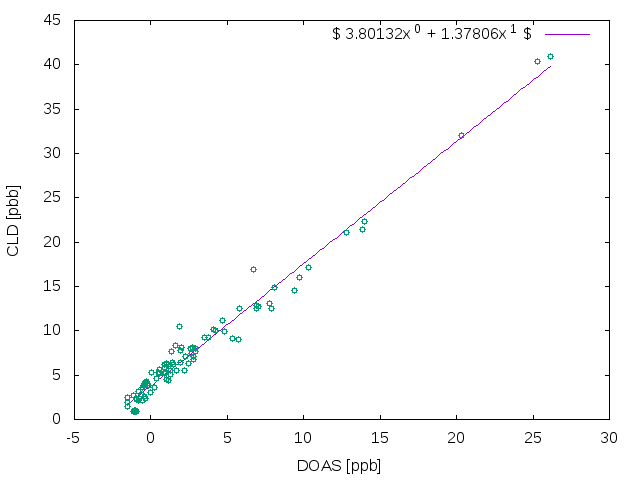
\includegraphics[width=0.7\textwidth]{20160122_25_fixI0_corr.png}
  % GNUPLOT: LaTeX picture with Postscript
\begingroup
  \makeatletter
  \providecommand\color[2][]{%
    \GenericError{(gnuplot) \space\space\space\@spaces}{%
      Package color not loaded in conjunction with
      terminal option `colourtext'%
    }{See the gnuplot documentation for explanation.%
    }{Either use 'blacktext' in gnuplot or load the package
      color.sty in LaTeX.}%
    \renewcommand\color[2][]{}%
  }%
  \providecommand\includegraphics[2][]{%
    \GenericError{(gnuplot) \space\space\space\@spaces}{%
      Package graphicx or graphics not loaded%
    }{See the gnuplot documentation for explanation.%
    }{The gnuplot epslatex terminal needs graphicx.sty or graphics.sty.}%
    \renewcommand\includegraphics[2][]{}%
  }%
  \providecommand\rotatebox[2]{#2}%
  \@ifundefined{ifGPcolor}{%
    \newif\ifGPcolor
    \GPcolorfalse
  }{}%
  \@ifundefined{ifGPblacktext}{%
    \newif\ifGPblacktext
    \GPblacktexttrue
  }{}%
  % define a \g@addto@macro without @ in the name:
  \let\gplgaddtomacro\g@addto@macro
  % define empty templates for all commands taking text:
  \gdef\gplbacktext{}%
  \gdef\gplfronttext{}%
  \makeatother
  \ifGPblacktext
    % no textcolor at all
    \def\colorrgb#1{}%
    \def\colorgray#1{}%
  \else
    % gray or color?
    \ifGPcolor
      \def\colorrgb#1{\color[rgb]{#1}}%
      \def\colorgray#1{\color[gray]{#1}}%
      \expandafter\def\csname LTw\endcsname{\color{white}}%
      \expandafter\def\csname LTb\endcsname{\color{black}}%
      \expandafter\def\csname LTa\endcsname{\color{black}}%
      \expandafter\def\csname LT0\endcsname{\color[rgb]{1,0,0}}%
      \expandafter\def\csname LT1\endcsname{\color[rgb]{0,1,0}}%
      \expandafter\def\csname LT2\endcsname{\color[rgb]{0,0,1}}%
      \expandafter\def\csname LT3\endcsname{\color[rgb]{1,0,1}}%
      \expandafter\def\csname LT4\endcsname{\color[rgb]{0,1,1}}%
      \expandafter\def\csname LT5\endcsname{\color[rgb]{1,1,0}}%
      \expandafter\def\csname LT6\endcsname{\color[rgb]{0,0,0}}%
      \expandafter\def\csname LT7\endcsname{\color[rgb]{1,0.3,0}}%
      \expandafter\def\csname LT8\endcsname{\color[rgb]{0.5,0.5,0.5}}%
    \else
      % gray
      \def\colorrgb#1{\color{black}}%
      \def\colorgray#1{\color[gray]{#1}}%
      \expandafter\def\csname LTw\endcsname{\color{white}}%
      \expandafter\def\csname LTb\endcsname{\color{black}}%
      \expandafter\def\csname LTa\endcsname{\color{black}}%
      \expandafter\def\csname LT0\endcsname{\color{black}}%
      \expandafter\def\csname LT1\endcsname{\color{black}}%
      \expandafter\def\csname LT2\endcsname{\color{black}}%
      \expandafter\def\csname LT3\endcsname{\color{black}}%
      \expandafter\def\csname LT4\endcsname{\color{black}}%
      \expandafter\def\csname LT5\endcsname{\color{black}}%
      \expandafter\def\csname LT6\endcsname{\color{black}}%
      \expandafter\def\csname LT7\endcsname{\color{black}}%
      \expandafter\def\csname LT8\endcsname{\color{black}}%
    \fi
  \fi
    \setlength{\unitlength}{0.0500bp}%
    \ifx\gptboxheight\undefined%
      \newlength{\gptboxheight}%
      \newlength{\gptboxwidth}%
      \newsavebox{\gptboxtext}%
    \fi%
    \setlength{\fboxrule}{0.5pt}%
    \setlength{\fboxsep}{1pt}%
\begin{picture}(7200.00,5040.00)%
    \gplgaddtomacro\gplbacktext{%
      \csname LTb\endcsname%
      \put(682,704){\makebox(0,0)[r]{\strut{}$0$}}%
      \put(682,1156){\makebox(0,0)[r]{\strut{}$5$}}%
      \put(682,1609){\makebox(0,0)[r]{\strut{}$10$}}%
      \put(682,2061){\makebox(0,0)[r]{\strut{}$15$}}%
      \put(682,2513){\makebox(0,0)[r]{\strut{}$20$}}%
      \put(682,2966){\makebox(0,0)[r]{\strut{}$25$}}%
      \put(682,3418){\makebox(0,0)[r]{\strut{}$30$}}%
      \put(682,3870){\makebox(0,0)[r]{\strut{}$35$}}%
      \put(682,4323){\makebox(0,0)[r]{\strut{}$40$}}%
      \put(682,4775){\makebox(0,0)[r]{\strut{}$45$}}%
      \put(814,484){\makebox(0,0){\strut{}$-5$}}%
      \put(1670,484){\makebox(0,0){\strut{}$0$}}%
      \put(2525,484){\makebox(0,0){\strut{}$5$}}%
      \put(3381,484){\makebox(0,0){\strut{}$10$}}%
      \put(4236,484){\makebox(0,0){\strut{}$15$}}%
      \put(5092,484){\makebox(0,0){\strut{}$20$}}%
      \put(5947,484){\makebox(0,0){\strut{}$25$}}%
      \put(6803,484){\makebox(0,0){\strut{}$30$}}%
    }%
    \gplgaddtomacro\gplfronttext{%
      \csname LTb\endcsname%
      \put(176,2739){\rotatebox{-270}{\makebox(0,0){\strut{}CLD [pbb]}}}%
      \put(3808,154){\makebox(0,0){\strut{}DOAS [ppb]}}%
    }%
    \gplbacktext
    \put(0,0){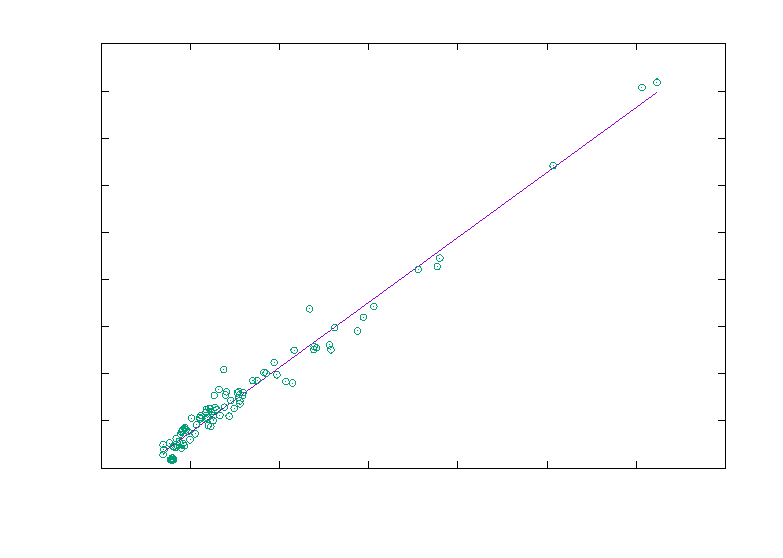
\includegraphics{../images/20160122_25_fixI0_corr}}%
    \gplfronttext
  \end{picture}%
\endgroup

  \caption{Correlation plot between our DOAS instrument and a
    chemiluminescence monitor (CLD). Each data point depicts a
    \SI{30}{\minute} average.}
  \label{fig:cld-corr}
\end{figure}


%%% Local Variables:
%%% mode: latex
%%% TeX-master: "../Bachelor"
%%% End:
